\section{The Path of Courtly Love}

\begin{quotex}
neither is the man without the woman, nor the woman without the man, in the Lord. \flright{\textsc{1 Corinthians 11:11}}

\end{quotex}

\begin{quotex}
There are few people who know the full strength of the different movements of the heart. The vast majority of men are sensitive to only five or six passions in the circle in which their lives are spent and which define the boundaries of their imaginations. Take away love and hate, pleasure and pain, hope and fear, and they will feel nothing. But persons of a nobler character can be moved in thousands of different ways. It seems that they can receive ideas and sensations which surpass the ordinary norms of the common people. \flright{\textsc{Abbe Prevost}, \emph{Manon Lescaut}}

\end{quotex}
There are many paths to God — the ways of the Monk, Ascetic, Mystic, Devotee, Sage. But the most effective, and little known, may be the Way of Courtly Love. This is the path of the Fedeli d'Amore, the Troubadour, the Alchemist, and the Knight Errant. The Muslim mystic, \textbf{Ibn Arabi}, was aware of this path:

\begin{quotex}
Contemplation of God without formal support is not possible… Since therefore some form of support is necessary, the best and most perfect kind is the contemplation of God in women. 

\end{quotex}

\begin{wrapfigure}{rt}{.3\textwidth}\centering
 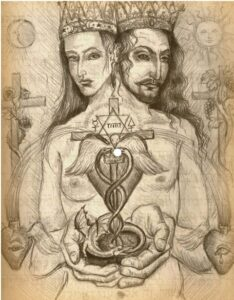
\includegraphics[scale=.6]{a20210207ThePathofCourtlyLove-img001.jpg} 
\caption{Androgyne}
\end{wrapfigure}

Formal manifestation, then, is the stepping stone to formless manifestation, and ultimately to the Supreme Identity. Hence, Dante had Beatrice and Ibn Arabi had Nizam to lead them upward. I have been aware of this path since I was a young man. Although following it often brings heartache, unfortunately even to the innocent, it is nonetheless effective. Herewith, we describe some preconditions and indicate some signposts to follow along the way.

\paragraph{Emotional Education}
In the decadent parts of the modern world, great attention is paid to physical and intellectual training, while emotional development is left entirely to chance. Sure, there is talk about “emotional intelligence”, which in practice achieves nothing. There are about a half dozen primary emotions, that can even be observed in babies: delight, fear, anger, surprise, discomfort, sadness. Over time, any developments in emotional responses are usually negative: anxiety, depression, worry, despair, self-doubt, inflation. That is why esoteric training begins with some preliminary objectives:

\begin{quotex}
The chief practical objectives are mastery of the sexual center, and the training of the emotional center. \flright{\textsc{Boris Mouravieff}, \emph{Gnosis}}

\end{quotex}
Emotional problems are obstacles to the Supreme Identity as they will disappear:

\begin{quotex}
The only things which have disappeared [in the unconditioned state] are the limiting conditions, which are negative, since they represent no more than a “privation”. \flright{\textsc{Rene Guenon}, \emph{Oriental Metaphysics [OM]}} 

\end{quotex}
Otherwise, the Supreme Identity is the fulfillment all of one's potentials in his other states:

\begin{quotex}
In this unconditioned state all other states of being find their place, but they are transformed and released from the special conditions which determined them as particular states. What remains is that which has a positive reality, since herein it is that all things have their own principle; the “delivered” being is truly in possession of the fullness of his own potentialities. \flright{\textsc{OM}}

\end{quotex}
What are these states? Tradition teaches that the Celestial Ray draws us upward. This vertical ray is perpendicular to the degrees of existence represented by successive planes. Death in one plane is birth in the next. Life then moves in a spiral around the Celestial Ray

\paragraph{Alchemical Marriage}
Since its goal is to achieve higher states beyond the merely biological, Alchemical Marriage requires mastery over the sexual center. In \emph{carnal love}, the couple becomes One Flesh. In \emph{Courtly Love}, the creative power of the sexual instinct leads to the couple being One Soul. In Tradition, this state is called the Androgyne. Guenon describes the necessary conditions:

\begin{quotex}
The union of complements must be regarded as constituting the primordial \textbf{Androgyne} of which all traditions speak. In the totalization of the being, the complements must in fact be in perfect equilibrium, with no predominance of one over the other. \flright{\textsc{Rene Guenon}, \emph{Symbolism of the Cross}}

\end{quotex}
There is no question of domination, as each soul reaches its full potential with no diminishment.

There is one precise woman and one precise man. However, when that is not possible there will be others that are “close enough”. Often, the couple may be geographically and temporarily separated, or one may even be deceased. Nevertheless, St. Paul assures us that no one is deprived (1 Corinthians 11:11).

\paragraph{Courtly Love}
\begin{quotex}
Courtly Love is the raison d'.tre for the couple of polar [i.e., complementary] beings: for the Knight and the Lady of his Dreams; without it, their polarity remains spiritualty sterile and they fall back into the common condition. Its practice, however, demands sacrifices and `exploits'. These are tests. For those who surmount them, the salutary effect of Gnosis is doubled: \emph{when it is enriched by experience, theoretical knowledge becomes living knowledge}. \flright{\textsc{Boris Mouravieff}}

\end{quotex}
Despite his artistic and scientific genius, Goethe failed to realize this courtly love in his ill-fated relationship with Ulrike. He treated her as common and ordinary. Nevertheless, unrequited love is not a failure, as Goethe then entered another creative period of his life. To the age-old question, “How do I know when I am in Love?” there is this answer:

\begin{quotex}
On all planes, the objective sign of Love's participation is the creative spirit which animates the subjects for whom it has become an aim. Conversely, if we think we are in Love but objectively do not notice an increase in creativity on any plane, either in ourselves or in our partner, we can be sure that the relationship is based on anything but Love. \flright{\textsc{Boris Mouravieff}}

\end{quotex}
\paragraph{The Union of Complements}
The descriptions of this contemplative union are usually one-sided. There are the well-known examples of Dante and Beatrice, Ibn Arabi and Nizam, Hafiz and the beautiful daughter, just to name a few. Some may claim that the women never physically existed, but Ibn Arabi denies it. What became, then, of the “real” Beatrice, the real Nizam, the daughter who become interested in Hafiz, just as he began his vigil. Don't they deserve a voice in the matter?

In other words, your polar being is not merely a prop for your spiritual development. In our state of being, she is as much flesh and blood as you are. She needs to be treated that way, since her own development is intertwined with yours.

I can share some personal experiences that may help you turn “theoretical knowledge” into “living knowledge”. Obviously, you wouldn't want to share the Supreme Identity with a stranger for all eternity, so you need to know your complementary or polar being.

A woman, at least the one that you should want, desires to be known, just as a man desires to know. It is important so pay attention to her, not just what she says, but more importantly what she means. Often, she does not even know herself, until it is articulated to her.

\paragraph{A Short Digression}
In the Turkish telenovela \emph{Sahsiyet}, the female character Nevra resists remembering the one thing that could free her from her life of promiscuity and inner turmoil. Agah, a government functionary his whole life, needs to come to terms with his impending death of his human person. He has been in position of the diary of a girl named Reyhan who was abused by the men of her village. He decides to become a Knight at that point, fights for justice for Reyhan and rescues the damsel Nevra. Agah knows her better that she knows herself, so he executes an elaborate plan that eventually allows Nevra to bring that hidden part of herself into conscious awareness; that liberates her.

\paragraph{Soul knowledge}
Sibylle surprisingly wrote: “To a woman the love of a man is incomprehensible.”\footnote{See Section~\ref{sec:NigredoAlbedoandRubedo} in this book.} Why would that be? If she is often pursued, she may be confused by the different motivations. If she feels herself to be unlovable, she may reject them all. The one mistake she can make is to assume that mere willfulness is a strength in itself. Then she may try to play the role of the Animus herself and become an ersatz man. Or else, she denies the Animus altogether and lives unconscious of her full potential. There is no way to reconcile those, so the double-mindedness can lead to doubt, division, confusion.

The Will must be guided by intelligence to be effective. Beatrice and Nizam are Wisdom, so they can pull Dante and Ibn Arabi upward along the Celestial Ray. In the world of flesh and blood, the woman supplies the man with the will to fight his battles. This is always a necessary component in the horizontal planes of existence that still include trial, conflict, and purgation. In exchange, she becomes who she truly is and is herself drawn up the Celestial Ray.

To write about the polar being only at the human, all-too-human, level will totally miss the point. Rather, it must be described from the states beyond the human state. Moreover, these must not be understood as merely psychological states.

What follows is a living, not theoretical, description, but don't assume it refers to a particular living person. It shows what to look for at the higher states of being. Bear in mind that the Person exists in all states simultaneously, even when unaware of them.

\paragraph{The Active Intellect}
Buddhi, or Active Intellect, is the first degree of the manifestation of the Androgyne. As such it is formless, not bound by individual conditions. Nevertheless, it is the father of the human intellect. Look, therefore, for someone of the same level of intelligence. While most people can only understand ideas that can be expressed in a slogan, she will have intellectual depth. Hence, she will be interested in high culture including art, poetry, music, mythology, psychology. Besides depth, she has a broad outlook that comes from knowledge of history and of different culture.

The lower intellect is the passive receptacle of ideas. Those in touch with the Active Intellect, on the other hand, are creators of ideas. She writes text. You share the same worldview to a large extent. You recognize the same landscape she creates, but her different perspective can be disorienting. But that is the motor force that drives the spiral up the Celestial Ray.

\paragraph{Manas}
After the Buddhi, Manas is the next degree; it begins to take individual form and is the principle of the individual senses and the organs of action. Manas is the inner sense. Our sensual awareness is not the creation of any physical or corporeal process. Otherwise, there could be no common experience, or experiences in other states of being.

Each of the five primary senses is related to one of the fundamental elements.

\paragraph{Vision}
There are many pretty girls, so what makes one more special than another? The vulgar will gaze at a woman's physical qualities, so you have the “ass man” or the “tit man”. But that is what women share in common, not what makes her unique. To find your Lady, you need to look for the features that set her apart and are meaningful only for you. They reveal more of her inner life than you might suppose.

As an example, look for qualities like these: The enigmatic color of her eyes, the way she cocks her head, her preference for angles rather than rectangles, her refusal to smile in photographs.

\begin{wrapfigure}{rt}{.45\textwidth}
 
\includegraphics[scale=.5]{a20210207ThePathofCourtlyLove-img002.jpg}
\end{wrapfigure} 

When you understand that the sense of Vision is associated with the Fire element, you will understand how the mere sight of her sets your heart ablaze. Sometimes it is can become physically painful so you have to look away. But you can't look away.

\paragraph{Voice}
Everything in the universe consists of vibrations, which are beyond matter and energy. Hence, the element Ether is associated with vibrations. It follows, then, that the auditory sense, which converts vibrations, arises with the Ether. Unlike the other gross elements, the Ether is subtle.

Her voice seems to arise from a transcendent source. The ancients understood this; they weren't bombarded with a cacophony of noise, so they understood silence. The voice of a Sybil rang true as a prophecy. Sometimes the allure was dangerous, like the tempting sons of the Sirens. But the voice of your Lady is only sweetness.

If you are fortunate, she will sing for you, and it will sound like the Music of the Spheres. Thanks to the gift of Memory, you can recall the song anytime you want.

\paragraph{Life is Bittersweet}
\begin{quotex}
In the Middle Ages, the Knight and his Lady, who considered themselves spiritually ONE did not venture into marriage. On the contrary, they parted, accepting the risk of never meeting again and knowing that if they did not triumph over a hard test, their love would degenerate, losing its meaning and its marvelous power. They knew that, by separating from each other for an \emph{exploit} they had a chance, while a premature marriage would be reduced to nothing. \flright{\textsc{Mouravieff}}
\end{quotex}

The legends of mythology and knightly valor know of these tests. Atalanta would only marry the one who could pass a test; but they allowed their passion to take old and were punished.

Often the exploit will take the Knight away. If he fails to return, they will need to wait for the next turn of the spiral to meet again. Just as they had promised each other in the previous turn. It sounds bittersweet, so I asked a sweet and insightful friend who explained:

\begin{quotex}
A little bittersweet. It is an art to take pleasure in sorrow. 

\end{quotex}
\paragraph{Appendix}
For more on Nizam, see The Lady Nizam — an Image of Love and Knowledge\footnote{\url{https://ibnarabisociety.org/the-lady-nizam-ralph-austin/}}.

William Anderson in \emph{Dante, The Maker} explains the influence of Beatrice on Dante:

\begin{quotex}
Through his love of her on Earth he formed an indissoluble union of love with her that transcended the incident of her death. She mirrored to him the Incarnation of Christ, and, in purifying his individual nature as a Christian, he found that the only way to the sight of God was through her as the revelation of his soul… so she, as his illuminated soul represents the search for unity and contains in herself the still causes of history and of creation. Through the love of her his love expands to become the love of God… she is in him the gateway to ecstatic joy. the source both of his inspiration and his salvation, the maker of him as a torch of living flame and his guide towards the peace which his difficult temperament and the sorrows of his bitter political life so long denied him. Through her guidance he achieved a total transformation in his emotional and intellectual being. 

\end{quotex}
Ibn Arabi describes his first meeting with Nizam, the daughter of a Persian scholar:

\begin{quotex}
Now this shaykh had a daughter, a lissome young girl who captivated the gaze of all those who saw her, whose mere presence was the ornament of our gatherings and startled all those who contemplated it to the point of stupefaction. Her name was Nizam (Harmonia) and her surname “Eye of the Sun and of Beauty”. Learned and pious, with an experience of spiritual and mystic life, she personified the venerable antiquity of the entire Holy Land and the candid youth of the great city faithful to the Prophet. Her glance, the grace of her conversation were such an enchantment… If not for the paltry souls who are over ready for scandal and predisposed to malice, I should comment here on the beauties of her body as well as her soul, which was a garden of generosity… And I took her as a model for the inspiration of the poems… although I was unable to express so much as a part of the emotion which my soul experienced and which the company of this young girl awakened in my heart, or of the generous love I felt… since she is the object of my quest and my hope, the Virgin most pure … 

\end{quotex}
Yet, his encounter with her, spiritually revealed a sharper aspect:

\begin{quotex}
One night I was performing the ritual circumambulations of the Ka'abah… suddenly a few lines of verse came to my mind. I recited them loudly enough to be heard… No sooner had I recited these verses than I felt on my shoulder the touch of a hand softer than silk. I turned around and found myself in the presence of a young girl, a princess from among the daughters of the Greeks. Never had I seen a woman more beautiful of face, softer of speech, more tender of heart. 

\end{quotex}


\flrightit{Posted on 2021-02-07 by Cologero }

\begin{center}* * *\end{center}

\begin{footnotesize}\begin{sffamily}



\texttt{Tannheuser on 2021-02-07 at 18:15 said: }

Thank you for this. I tried living without Love for a long time, finding it again was transformative. One of the reasons it is such an “effective” path is the way Love easily burns away many bad habits and impurities of the senses that can be difficult to master otherwise.

On the other hand, Love is bittersweet as you say, and involves very painful tests of all kinds. Every kind of meeting with the Beloved, no matter how sweet, involves a departure, and has the double character of requiring excruciating restraint and control of oneself – the ability to stand firm and not be swept away by the whirlwind described in Inferno Canto V, that beats from all sides.

Of the Will that a woman provides a man to fight his battles, take the example of Palomides in Malory, who is powerfully inspired by Isoud, despite his love being unrequited:

—

“Sir Palomides looked up toward her where she [Isoud] lay in the window, and he espied how she laughed; and therewith he took such a rejoicing that he smote down, what with his spear and with his sword, all that ever he met; for through the sight of her he was so enamoured in her love that he seemed at that time, that an both Sir Tristram and Sir Launcelot had been both against him they should have won no worship of him; and in his heart, as the book saith, Sir Palomides wished that with his worship he might have ado with Sir Tristram before all men, because of La Beale Isoud. Then Sir Palomides began to double his strength, and he did so marvellously that all men had wonder of him, and ever he cast up his eye unto La Beale Isoud. And when he saw her make such cheer he fared like a lion, that there might no man withstand him; and then Sir Tristram beheld him, how that Sir Palomides bestirred him; and then he said unto Sir Dinadan: So God me help, Sir Palomides is a passing good knight and a well enduring, but such deeds saw I him never do, nor never heard I tell that ever he did so much in one day.

…

Well, said Dinadan to himself, all this worship that Sir Palomides hath here this day he may thank the Queen Isoud, for had she been away this day Sir Palomides had not gotten the prize this day.

…

Well, said Sir Launcelot, I see, for to say thee sooth, ye have done marvellously well this day; and I understand a part for whose love ye do it, and well I wot that love is a great mistress. And if my lady were here as she nis not, wit you well, said Sir Launcelot, ye should not bear away the worship.”

(Mort d'Arthur Book X, Ch. LXX)


\hfill

\texttt{Paulo Adolpho on 2021-02-07 at 22:38 said: }

“There are many pretty girls, so what makes one more special than another? The vulgar will gaze at a woman's physical qualities, so you have the “ass man” or the “tit man”. But that is what women share in common, not what makes her unique. To find your Lady, you need to look for the features that set her apart and are meaningful only for you. They reveal more of her inner life than you might suppose.As an example, look for qualities like these: The enigmatic color of her eyes, the way she cocks her head, her preference for angles rather than rectangles, her refusal to smile in photographs.”

“In the Middle Ages, the Knight and his Lady, who considered themselves spiritually ONE did not venture into marriage. On the contrary, they parted, accepting the risk of never meeting again and knowing that if they did not triumph over a hard test, their love would degenerate, losing its meaning and its marvelous power. They knew that, by separating from each other for an exploit they had a chance, while a premature marriage would be reduced to nothing. \flright{\textsc{Mouravieff”}}

These parts above, summarize the true understanding, the essential knowledge, on this issue. And what about you Cologero, do you have experienced what is described above?


\hfill

\texttt{Tannheuser on 2021-02-09 at 21:53 said: }

“In other words, your polar being is not merely a prop for your spiritual development. In our state of being, she is as much flesh and blood as you are. She needs to be treated that way, since her own development is intertwined with yours.

…

A woman, at least the one that you should want, desires to be known, just as a man desires to know. It is important so pay attention to her, not just what she says, but more importantly what she means. Often, she does not even know herself, until it is articulated to her.”

—

In the modern world, this is painful. Allowing oneself to love a woman today feels a little like what it must be like for Christ to love the world. Her spiritual well-being becomes my concern, and suddenly all of the awful decisions she makes are harmful to me also. The Garden of Gethsemane is the first thing that comes to my mind here. Like the Elves who leave Middle-earth for the Undying Lands, there's a part of me that also wants to leave it all.

In the human state, I think it is possible only to really love one other person in this way. I think it requires angelic and higher states of consciousness in order to really love beyond that, and the first love is the gateway to everything else. Universal love that is not based on these higher states of being, on the other hand, is a counterfeit.


\hfill

\texttt{Tyler on 2021-02-09 at 22:09 said: }

On the subject of artistry, romanticism, and the Path of Courtly Love, can you speak in some way to this strange importance I perceive of *not* breaking the fourth wall? I don't quite grasp it in full as I am still young.

A magician never reveals his secrets – but in some way I feel I would go insane if I never broke the fourth wall with my lady. Which is it? Does this make sense?


\hfill

\texttt{Cologero on 2021-02-09 at 22:46 said: }

Yes, you and your lady are starring in the same film together, but as characters. To break the fourth wall is to become the actor in the film, not just the character; the audience as well as the players. It is complex. A similar idea is developed in Gnosis Book One on the topic of the “film” of life. But to start there, in media res, will be difficult probably.


\hfill

\texttt{Isma'il on 2021-08-26 at 01:36 said: }

Peace friends,

“In the modern world, this is painful. Allowing oneself to love a woman today feels a little like what it must be like for Christ to love the world. Her spiritual well-being becomes my concern, and suddenly all of the awful decisions she makes are harmful to me also. The Garden of Gethsemane is the first thing that comes to my mind here. Like the Elves who leave Middle-earth for the Undying Lands, there's a part of me that also wants to leave it all.”

My sympathies. Qur'anic exotericisms on marriage conditions are very useful. A woman entering into marriage aware that:

– he can marry others, but she cannot, though divorce is normal

– while married, he has the right to physically spank her should vanity overcome obedience

– many others

…are all a deep Mercy I think, especially for this time. 

Don't worry about classical Fiqh, it is full of things that don't make sense in our age. At the danger of being Protestant, taking the Quranite approach of seeing it as the complete independent revelation that it claims to be clears a lot of that mess.

Salaam.


\hfill

\texttt{Mail on 2021-08-29 at 08:16 said: }

A little interesting, Isma'il, that you invoke the Qu'ranic teaching on disciplining women but then tell us not to worry about fiqh. Most of us readers here at Gornahoor are living in countries where we are temporally judged by a modern legal system not based on fiqh, and that includes our decisions on how to handle women.

Because of this, most of us have had an intuition of the Western path of courtly love. It underlies the expectations of this modern system, so being raised in the system, and desiring to know the truth mixed with its lies, we are slowly directed towards that path. You may find that when you meet your Muslim beauty, your Western intuition provides you with an orientation that her other suitors have lacked, and you will feel safe to walk the path of life with her out of a shared hunger for the soul as Cologero writes about here, without desiring a moral basis for physical domination. But it seems to me you must also take care in the way you think about fiqh, as religious syncretism engenders modernism.


\hfill

\texttt{Marcellus on 2022-07-23 at 21:10 said: }

I thought to myself last night that I had seen god. I had focused strongly on one who is indifferent to me and how I could be with her, and the potentialities were shown to me, and I witnessed the higher plane of love in estastic vision. I had seen Dante's vision, I said. At one time, I was filled with the greatest warmth from the fire within, and I shed tears in awe. Alas, she was but “good enough”, I can only assume, for I know her not well. I was only truly brought back down to reality a few hours later from a manosphere video.


\end{sffamily}\end{footnotesize}
